% Created 2020-09-18 ven. 09:30
% Intended LaTeX compiler: pdflatex
\documentclass[justified]{tufte-handout}
 \usepackage{multicol}
\usepackage{units}
\usepackage[french, english]{babel}

  \usepackage{graphicx}
  \usepackage[colorlinks=true]{hyperref}
\author{Maxime Cochennec}
\date{\today}
\title{Vérification calcul pressure drag}
\hypersetup{
 pdfauthor={Maxime Cochennec},
 pdftitle={Vérification calcul pressure drag},
 pdfkeywords={},
 pdfsubject={},
 pdfcreator={Emacs 26.3 (Org mode 9.3.6)}, 
 pdflang={English}}
\begin{document}

\maketitle
\tableofcontents



\section{Problème}
\label{sec:org62e5345}

On cherche à calculer l'intégrale \footnote{La composante selon \(x\) de l'intégrande est nul si symétrie
d'axe \(y\). Dans le cas d'une double symétrie d'axe \(x\) et \(y\), par
ex. une bulle parfaitement cylindrique, l'intégrande est nul.}
\begin{equation}\label{eq:int}
\frac{1}{S}\int_{\Gamma_{wo}}\gamma\left(\frac{\pi}{4}\kappa_{\parallel}-\frac{2}{h}\cos\theta\right)\mathbf{n}_{ow}  \:\mathrm{d}l,
\end{equation}
en particulier on s'intéresse à la composante selon \(x\) afin de
discuter la différence entre les forces de trainées \(d_{ow} \vert_x -
d_{wo}\vert_x\).


\vspace{0.8cm}
\noindent
L'intégrale \ref{eq:int} est calculée en
dehors de Comsol comme suit :
\begin{itemize}
\item export de l'interface,
\item reconstruction par fitting avec un polynôme,
\item calcul sur l'interface reconstruite.
\end{itemize}
\noindent
On note que
\begin{equation}
\int_{\Gamma_{wo}}(p_{w}-p_{o})\mathbf{n}_{ow}\cdot\mathbf{e}_{x}\:\mathrm{d}l=\int_{\Gamma_{wo}}\gamma\left(\frac{\pi}{4}\kappa_{\parallel}-\frac{2}{h}\cos\theta\right)\mathbf{n}_{ow}\cdot\mathbf{e}_{x}\:\mathrm{d}l,
\end{equation}
\noindent puisque la viscosité des fluides est identique. On vérifie
d'abord que l'intégrale \ref{eq:int} est bien nulle dans le cas d'une
interface avec une symétrie d'axe \(y\). Ensuite, on présente les résultats.

\section{Vérification avec interface symétrique}
\label{sec:org7ecbd00}

\begin{marginfigure}
  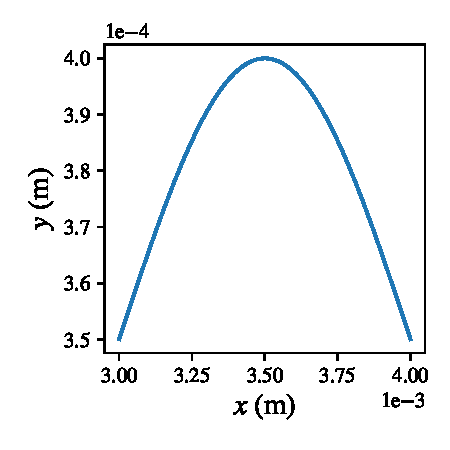
\includegraphics[width=\linewidth]{symInt.pdf}
  \caption{Interface symétrique utilisée pour l'exemple.}
  \label{fig:marginfig1}
\end{marginfigure}

On utilise une interface symétrique (Fig.\ref{fig:marginfig1}) afin de
vérifier si le calcul de l'intégrale \ref{eq:int} renvoie bien un
résultat nul. Les résultats sont donnés dans la Table
\ref{tab:org7327f8c}. L'intégrale est bien nulle.

\begin{table}[htbp]
\caption{\label{tab:org7327f8c}Courbure moyenne dans le plan et résultat de l'intégrale pour l'interface symétrique Fig.\ref{fig:marginfig1}}
\centering
\begin{tabular}{rl}
\(\langle \kappa\)\textsubscript{\(\parallel\)}\(\rangle\) (1/m) & Intégrale (N/m)\\
\hline
-308 & 3\texttimes{}10\textsuperscript{-17}\\
\end{tabular}
\end{table}

\section{Résultats}
\label{sec:org88b19f6}
On calcule maintenant la courbure moyenne et l'intégrale \ref{eq:int}
en fonction de l'entrefer et pour deux nombres capillaire. Les
résultats sont donnés dans les Tables \ref{tab:orge94ce7b} et \ref{tab:org961c12c}. 

\begin{table}[htbp]
\caption{\label{tab:orge94ce7b}Courbure moyenne dans le plan et résultat de l'intégrale en fonction de l'entrefer (\(Ca=0.5\)).}
\centering
\begin{tabular}{rrrrr}
\(h^*\) & \(\langle \kappa\)\textsubscript{\(\parallel\)}\(\rangle\) (1/m) & Intégrale (N/m\textsuperscript{3}) & \(\int \mathbf{n} \cdot \mathbf{e}_x \: \mathrm{d} l\) & \(d_{ow}\) (N/m\textsuperscript{3})\\
\hline
5 & 25 & -4.65e-3 & -2.79E-06 & 15.2\\
2 & 29 & -1.83e-3 & -3.21E-06 & 16.3\\
1 & 33 & 8.54e-3 & -4.90E-06 & 21.2\\
0.5 & 39 & 3.44e-2 & -5.92E-06 & 43.7\\
0.25 & 43 & 6.05e-2 & -4.26E-06 & 138.5\\
0.125 & 53 & 5.05e-2 & -1.67E-06 & 490.2\\
0.05 & 60 & 7.28e-2 & -9.24E-07 & 2484.0\\
\end{tabular}
\end{table}

\begin{table}[htbp]
\caption{\label{tab:org961c12c}Courbure moyenne dans le plan et résultat de l'intégrale en fonction de l'entrefer (\(Ca=0.025\)).}
\centering
\begin{tabular}{rrrrr}
\(h^*\) & \(\langle \kappa\)\textsubscript{\(\parallel\)}\(\rangle\) (1/m) & Intégrale (N/m\textsuperscript{3}) & \(\int \mathbf{n} \cdot \mathbf{e}_x \: \mathrm{d} l\) & \(d_{ow}\) (N/m\textsuperscript{3})\\
\hline
5 & -11 & 2.48e-2 & 3.70E-05 & 13.3\\
2 & -12 & -2.84e-4 & 2.96E-05 & 13.5\\
1 & -17 & 1.00e-1 & 2.14E-07 & 14.6\\
0.5 & -23 & 6.10e-1 & -4.55E-05 & 24.0\\
0.25 & -1 & 5.93e+0 & -2.93E-04 & 109.9\\
0.125 & 56 & 1.31e+1 & -3.61E-04 & 431\\
0.05 & 61 & 8.32e+0 & -1.07E-04 & 2502\\
\end{tabular}
\end{table}

\noindent Les résultats de l'intégrale \ref{eq:int} sont très petits
au regard de la force de trainée calculée dans le papier. Ces
résultats confirment le résultat du papier, c-à-d, \(d_{ow} \vert_x \approx
d_{wo}\vert_x\).


\begin{figure}
  \centering
  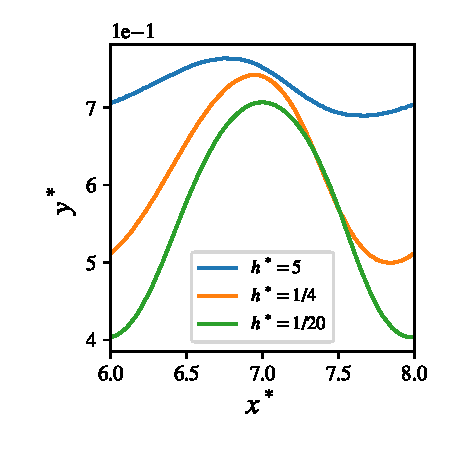
\includegraphics[width=0.8\linewidth]{Int.pdf}
  \caption{Position de l'interface fluide-fluide en fonction de l'entefer pour $Ca=0.025$. Une symétrie
  d'axe $y$ apparaît pour un entrefer très petit.}
  \label{fig:Int}
\end{figure}


\begin{figure}
  \centering
  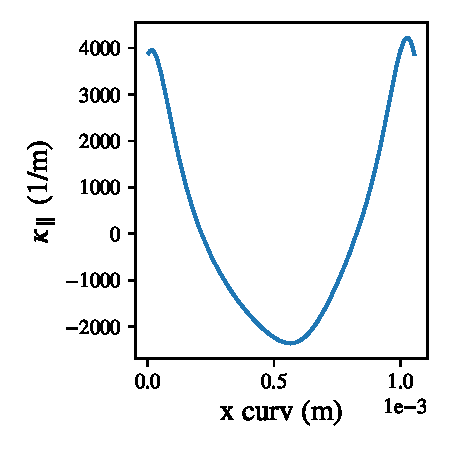
\includegraphics[width=0.8\linewidth]{kappa.pdf}
  \caption{Courbure dans le plan de l'interface le long de son abscisse curviligne ($Ca=0.025$ et $h^*=1/20$).}
  \label{fig:marginkappa}
\end{figure}


\clearpage
\section{Code}
\label{sec:orgc0eea86}
\begin{verbatim}
import matplotlib
import numpy as np
matplotlib.use("Agg")
import matplotlib.pyplot as plt
from matplotlib import rc
from scipy.optimize import curve_fit
from scipy.integrate import trapz

matplotlib.rcParams["mathtext.fontset"] = "stix"
matplotlib.rcParams["font.family"] = "STIXGeneral"

# constant
#gamma = 2.23e-6
h = 5e-4 * 0.05
Surf = 5e-4 * 1e-3
gamma = 4.46e-5

xReconstruct = np.linspace(3e-3, 4e-3, num=100000)

# artificial symmetric interface
yArtificial = -5e-5 * np.sin(xReconstruct * np.pi / 1e-3) + 3.5e-4

xy = np.array(data, float)
z = np.polyfit(xy[:, 0], xy[:, 1], 8)
yReconstruct = np.polyval(z, xReconstruct)

# ----COMPUTE GRADIENT
dx = np.gradient(xReconstruct)
ddx = np.gradient(dx)
dy = np.gradient(yArtificial)
ddy = np.gradient(dy)

# ----COMPUTE NORMAL VECTOR
nx = np.divide(-dy, np.sqrt(dx ** 2 + dy ** 2))
ny = np.divide(dx, np.sqrt(dx ** 2 + dy ** 2))

# ----COMPUTE ELEMENT LENGTH
ds = np.sqrt(dx ** 2 + dy ** 2)
sumds = np.cumsum(ds)

# ----COMPUTE CURVATURE
num = np.multiply(dx, ddy) - np.multiply(ddx, dy)
denom = (np.multiply(dx, dx) + np.multiply(dy, dy)) ** (3 / 2)

kappa = np.divide(num, denom)

L = np.sum(ds)

intnx = trapz(nx[2:-2], xReconstruct[2:-2])
intny = trapz(ny[2:-2], xReconstruct[2:-2])

meankappa = trapz(kappa[2:-2], xReconstruct[2:-2]) / L
meankappa1 = np.sum(np.multiply(kappa, ds)) / L

integral = gamma * trapz(nx[2:-2] * (kappa[2:-2] * np.pi / 4 - (2 / h)), xReconstruct[2:-2]) / Surf
integralnx = gamma * trapz(nx[2:-2], xReconstruct[2:-2]) / Surf 
plt.clf()

fig1 = plt.figure(figsize=(3, 3))
plt.plot(xReconstruct[2:-2], yArtificial[2:-2])
plt.xlabel(r"$x$ (m)", fontsize=14)
plt.ylabel(r"$y$ (m)", fontsize=14)
plt.ticklabel_format(axis="x", style="sci", scilimits=(0, 0))
plt.ticklabel_format(axis="y", style="sci", scilimits=(0, 0))
fig1.tight_layout()
# plt.savefig('symInt.pdf')
plt.close()

fig2 = plt.figure(figsize=(3, 3))
plt.plot(sumds[3:-3],kappa[3:-3])
plt.xlabel(r'x curv (m)',fontsize=14)
plt.ylabel(r'$\kappa_{\parallel}$ (1/m)',fontsize=14)
plt.ticklabel_format(axis="x", style="sci", scilimits=(0, 0))
fig2.tight_layout()
#plt.savefig('kappa.pdf')

print("%2d,%2d,%10.2E,%10.2E"% (meankappa,meankappa1,integral,integralnx))
\end{verbatim}
\end{document}